%\addcontentsline{toc}{chapter}{Kapitel-1}
\chapter{Bibliotheken/Software}

In diesem  Abschnitt werden einige Möglichkeiten zur Erkennung von Partikeln in einem Video niedriger Auflösungsqualität verglichen und hervorgehoben. Es wäre natürlich ideal einen Vergleich zwischen manuellen und werkzeugbasierten Erkennung zu ziehen. Aber leider wird die manuelle Erkennung hier nicht vollzogen aufgrund der viel zu schwierig bzw. langwierige Arbeit, die es bereitet. Es geht hier nämlich um mehrere hunderte von Partikeln pro Bild.\\
 
\begin{figure}[H]
    \centering
    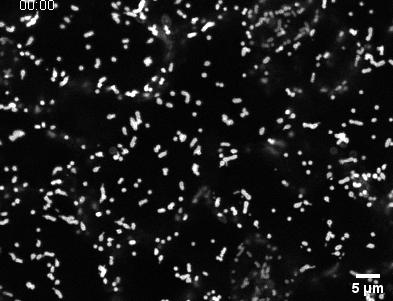
\includegraphics[scale=0.9]{Grafiken/trackpyBilder/video-frame00001.png}
    \caption{raw image with particles to be detected}
    \label{fig:bild_label}
\end{figure}

In diesem Sinne widmet sich die Arbeit in der Folgezeit dem Vergleich möglicher Werkzeugen, die zur Erreichung der eigentlichen Ziele nutzen können. Hierbei werden aus der Vielzahl der Instrumente nur vier bis fünf herausgegriffen. Diese werden zunächst einer tabellarischen Grobanalyse der Merkmale und dann einer textuellen Analyse der Unterschiede unter ihnen unterzogen.\\

\todo{ ToDo: Zwei weitere Partikel-Tracking-Bibliotheken finden.}
\todo{ ToDo: Eigenschaften jeglicher Tool im Vergleich Anderer zu herausfinden}

\begin{tabular}{|c||c|c|l|}
\hline
Werkzeug & Schwerpunkt & Zugänglichkeit & Parameteranzahl \\
\hline
\hline
 ParticleTracker & & & \\
 \hline
 PyPIV   & & & \\
 \hline
 OpenPTV & & & \\
 \hline
 STracking  & & & \\
 \hline
 PySTACHIO  & & & \\
 \hline
 TrackPy  & & & \\
 \hline
\end{tabular}
\\

\todo{\href{file:///C:/Users/leb/Downloads/10.21105.joss.04398.pdf}{MyPTV}, \\ \href{https://www.sciencedirect.com/science/article/pii/S2001037021002944}{PySTACHIO},\\ \href{https://spt.readthedocs.io/en/latest/}{SPT}
\\ \href{https://www.google.com/search?q=Python+package+for+particle+tracking&rlz=1C1CHBF_deDE987DE987&sxsrf=ALiCzsYl2NtGnlFYYupES17uNyNLp8zhIQ:1653590912505&ei=gMuPYoKwHsyMxc8Phquk2AM&start=10&sa=N&ved=2ahUKEwiC8MWX6v33AhVMRvEDHYYVCTsQ8NMDegQIARBQ&biw=1920&bih=969}{Python package for particle tracking}}

\section{ParticleTracker}
\textbf{ParticleTracker} ist eine vollständig grafisch bedienbare Software, die es erlaubt, Partikel aus einem Video guter oder niedriger Auflösung zu verfolgen. Diese verwendet mehrere verschiedene Verfolgungsalgorithmen mit einer Standardschnittstelle, um die Einrichtung verschiedener Partikelverfolgungsprojekte schnell und einfach zu gestalten \cite{Smith2021}.
Es werden 3 Methoden des "Tracking" verwendet, nämlich:
\textit{Opencv Hough Circles}: zum Auffinden von Kreisen in einem Bild.
\textit{Trackpy}: Eine bestehende Partikelverfolgungsbibliothek zur Verfolgung von Partikel 
\textit{Opencv Contour finding}: Zum Finden von Konturen in einem Binärbild.
Das erste und das letzte werden von OpenCV \cite{opencv_library} bereitgestellt.

	\paragraph{Vorteile}
		\begin{enumerate}
    			\item \textbf{GUI bedienbar}: \\
				Die Benutzeroberfläche ist eine der beliebtesten Arbeitsmethoden für Benutzer, insbesondere für Neulinge(Siehe \cite{hertzum1996browsing}). Dies ist sicherlich eine hervorragende Möglichkeit, in diesen Bereich einzusteigen, ohne sich mit zu vielen Codezeilen auseinandersetzen zu müssen oder Programmierkenntnisse zu besitzen.
				
    			\item \textbf{Anfängerfreundlich}:\\
				Die Anfängerfreundlichkeit ist stark auf den vorherigen Punkt zurückzuführen, nämlich die GUI-Bedienbarkeit. Zudem ist es sonderlich umstandslos, mit Hilfe einiger Klicks, sich Informationen generieren zulassen, die relevant sind.    
				
    			\item \textbf{Datenvisualisierung}:\\
    			Ein großer Vorteil ist Datenvisualisierung. Dies liegt an der schrittweisen und automatischen Aktualisierung des Renderings in Abhängigkeit von den vorgenommenen Einstellungen. Allerdings ist es notwendig, zunächst das Kästchen "Annotate" zu aktivieren, um die Live-Ansicht zu aktivieren.
    			
    			\item \textbf{Datenausgabe}:\\
 				Der Zugang zu den Daten in der Software ist schnell und einfach. Außerdem sind die Daten in verschiedenen Formen verfügbar. Unter anderem werden die Daten als csv-Datei und auch als Video bereitgestellt, das die Entwicklung der Objekte im Ausgangsvideo nachzeichnet. 
Es ist auch wichtig zu erwähnen, dass es möglich ist, die Daten (in csv) in Bezug auf ein einzelnes Bild zu exportieren.
		\end{enumerate}
		
	\paragraph{Nachteile}
		\begin{enumerate}
				\item \textbf{Das Hochfahren der Software}:\\
				Trotz der Dokumentation war es nicht einfach, die Software zum Laufen zu bringen. In Anbetracht der Verwendung von Bibliotheken, die nur in einer bestimmten Python-Umgebung  verfügbar sind, nämlich "Conda".
Daher wäre es fair zu erwähnen, dass dies für Laien noch schwieriger sein könnte.
				
    			\item \textbf{Funktionsbegrenzt}:\\
				Die Benutzung über eine GUI ist zwar begeisternder Punkt. Doch genau hier liegt die Schwäche. Da die Benutzeroberfläche bereits konfiguriert ist, bietet sie nur die Möglichkeit, die verfügbaren Optionen zu nutzen. Dies könnte in manchen Fällen zu einem Mangel an Optionen führen und somit unzureichend sein.    			
    			
    			\item \textbf{Nicht intuitiv}:\\
    			Obwohl die Verwendung einer grafischen Oberfläche im Allgemeinen für den Benutzer attraktiver ist, sollte sie so intuitiv wie möglich sein oder gut dokumentiert werden (zumindest als Tooltip).
In diesem Fall sind die Namen einiger Optionen auf der Schnittstelle nicht sehr aussagekräftig oder beschreibend(siehe Bild).
\begin{figure}[H]
    \centering
    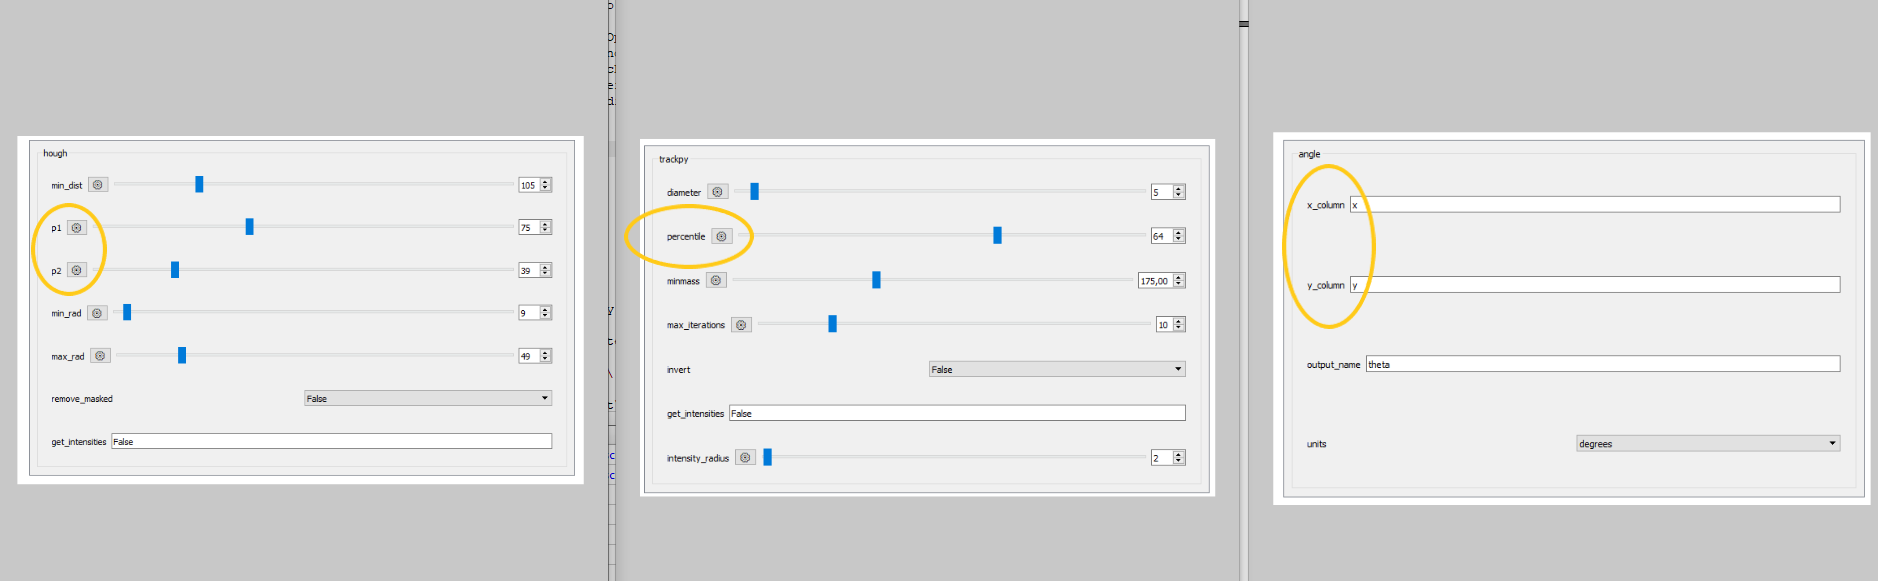
\includegraphics[scale=0.35]{Grafiken/particletracker/Not intuitive.png}
    \caption{Poorly described option names}
    \label{fig:bild_label}
\end{figure}
Es ist daher verständlich, dass man Hinweise erwartet, die die Verwendung der Optionen (Schaltflächen) im Detail beschreiben. 
Dies ist leider nicht der Fall. Daher erfordert die Benutzung der Software ein gewisses Hin und Her in der externen Dokumentation, um die Rolle der Optionen zu kennen.
		\end{enumerate}
		
	\paragraph{Beispiel}
	Wir zeigen hier ein Beispiel für die Erkennung von Partikeln auf einem bestimmten Bild.
	 
	\begin{figure}[H]
    \centering
    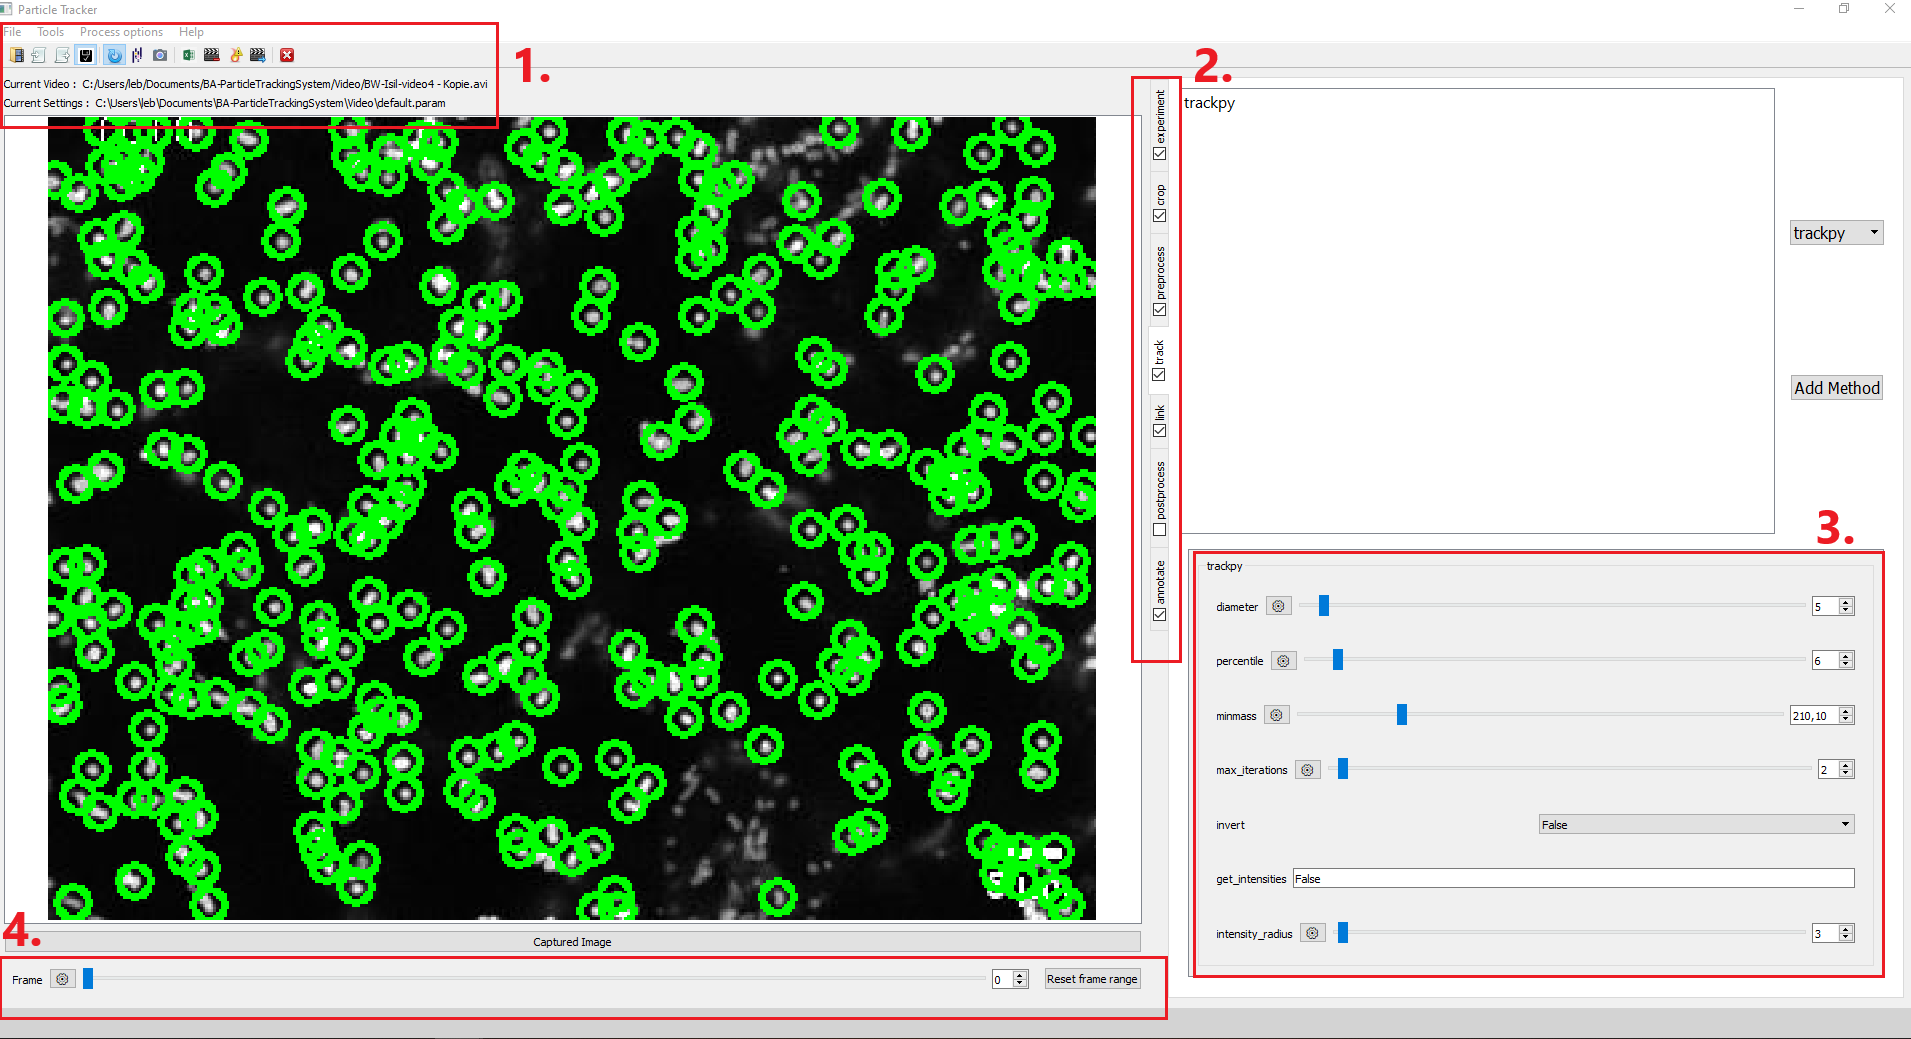
\includegraphics[scale=0.3]{Grafiken/particletracker/Using trackpy.png}
    \caption{Example of particle detection using Trackpy-method of particleTracker}
    \label{fig:bild_label}
\end{figure}

\newpage
	
\section{PyPTV}
\textbf{PyPTV} ist ...

	\paragraph{Vorteile}
		\begin{enumerate}
    			\item raw\_image: array \\

    			\item diameter: odd integer \\

    			\item minmass: float \\
    			
    			\item separation: float\\
 			
    			\item max\_iterations: interger\\
    			
		\end{enumerate}
		
	\paragraph{Nachteile}
		\begin{enumerate}
    			\item raw\_image: array \\

    			\item diameter: odd integer \\

    			\item minmass: float \\
    			
    			\item separation: float\\
 			
    			\item max\_iterations: interger\\
    			
		\end{enumerate}
		
	\paragraph{Beispiel}

\section{OpenPTV}
\textbf{OpenPTV} ist ... 

	\paragraph{Vorteile}
		\begin{enumerate}
    			\item raw\_image: array \\

    			\item diameter: odd integer \\

    			\item minmass: float \\
    			
    			\item separation: float\\
 			
    			\item max\_iterations: interger\\
    			
		\end{enumerate}
		
	\paragraph{Nachteile}
		\begin{enumerate}
    			\item raw\_image: array \\

    			\item diameter: odd integer \\

    			\item minmass: float \\
    			
    			\item separation: float\\
 			
    			\item max\_iterations: interger\\
    			
		\end{enumerate}
		
	\paragraph{Beispiel}

\section{STracking}
\textbf{STracking} ist ... 

	\paragraph{Vorteile}
		\begin{enumerate}
    			\item raw\_image: array \\

    			\item diameter: odd integer \\

    			\item minmass: float \\
    			
    			\item separation: float\\
 			
    			\item max\_iterations: interger\\
    			
		\end{enumerate}
		
	\paragraph{Nachteile}
		\begin{enumerate}
    			\item raw\_image: array \\

    			\item diameter: odd integer \\

    			\item minmass: float \\
    			
    			\item separation: float\\
 			
    			\item max\_iterations: interger\\
    			
		\end{enumerate}
		
	\paragraph{Beispiel}

%\addcontentsline{toc}{section}{Kapitel-1}
%\section{Werkzeugbasierte Erkennung}
\section{Trackpy}
Trackpy ist ein Python-Paket, das es ermöglicht aus einem Video bzw. einer Imagesequenz Partikel in unterschiedlichen Dimensionen (2D und 3D) zu erkennen und zu verfolgen. Hier wird es natürlich die Zweidimensionalität anvisiert. Die Erkennung der Partikel erfolgt über eine der Funktionen des Paketes, nämlich die \textit{locate-}Funktion.
Dieser verfügt über eine reihe von Parametern, anhand derer die Qualität der Anerkennung ausgebessert werden kann.

	\paragraph{Vorteile}
		\begin{enumerate}
    			\item raw\_image: array \\

    			\item diameter: odd integer \\

    			\item minmass: float \\
    			
    			\item separation: float\\
 			
    			\item max\_iterations: interger\\
    			
		\end{enumerate}
		
	\paragraph{Nachteile}
		\begin{enumerate}
    			\item raw\_image: array \\

    			\item diameter: odd integer \\

    			\item minmass: float \\
    			
    			\item separation: float\\
 			
    			\item max\_iterations: interger\\
    			
		\end{enumerate}
		
	\paragraph{Beispiel}

\todo{kapitel1: Which  Library to use(avaible/)
kap2: Choosing good parameters for trackpy
kap3(Main Challenge):The Challenge of keeping particle count constant over frames.}

